\documentclass[11pt,a4paper]{article}
\usepackage[utf8]{inputenc}\usepackage[T1]{fontenc}
\usepackage[margin=1in]{geometry}
\usepackage{amsmath,amssymb,booktabs,graphicx,enumitem,xcolor,parskip,titlesec}
\usepackage[hidelinks]{hyperref}
\graphicspath{{figures/}}
\definecolor{qnavy}{RGB}{20,40,75}\definecolor{qgrey}{RGB}{90,90,90}
\definecolor{qred}{RGB}{150,30,30}\definecolor{qgreen}{RGB}{47,107,79}
\titleformat{\section}{\large\bfseries\color{qnavy}}{\thesection}{0.6em}{}
\begin{document}\thispagestyle{empty}
\noindent
{\large\bfseries\color{qnavy} Report R18 --- Archive or Encoder?}\\[2pt]
{\color{qgrey}Paper 1's first limitation was that every site-leakage number came from
Phikon-v2 features. This re-runs the whole measurement over a second encoder that has never seen
histology.}\\[6pt]
{\color{qgrey}\rule{\textwidth}{0.4pt}}

\medskip
\noindent 17 August 2026 \quad\textbullet\quad Quantara \quad\textbullet\quad
{\color{qgrey}Peer-review audit copy}

\medskip
\noindent{\small\color{qgrey}\emph{Every number in this report is substituted from
\texttt{evidence/results.json} by \texttt{make\_report.py}. Nothing is typed by hand. This is
the response to R19, where two manuscript numbers had no artefact behind them and the verification
pass confirmed them against memory.}}

\section*{Summary}

R12--R15 measured a large site signature in whole-slide features: subtype AUROC inflates by
+0.1710 and the six methylation targets by +0.0849 in
mean $\rho$ when cross-validation folds share tissue-source sites instead of holding them out.
Every one of those numbers came from Phikon-v2. The obvious objection is that pan-cancer histology
pretraining might encode institutional stain and scanner character, in which case the finding is
about Owkin's model and not about federated pathology.

This report re-runs the identical measurement over \texttt{facebook/dinov2-large}: the same
\texttt{Dinov2Model} class, the same 1024-dimensional width, the same 24 layers, the same DINOv2
self-supervision, the same CLS-token readout and the same ImageNet normalisation --- trained on
natural images rather than histology. The tile grids are byte-identical between the two feature
sets, verified on slides spanning 887 to 28{,}666 tiles, so the encoder is the only thing that
differs.

\textbf{Verdict: SITE\_SIGNATURE\_IS\_ARCHIVE\_NOT\_ENCODER}. The site signature is a property of the archive, not of Phikon-v2. It reproduces under an encoder that has never seen a histology slide, so Paper 1's claim is about federated pathology rather than about one vendor's model.

\section{The controls came first}

A comparison across encoders is worthless if the harness is not the one that produced the
published numbers, so the Phikon-v2 arms were re-run through the new harness and gated against
R15 before the second encoder was allowed to count.

\begin{center}
\begin{tabular}{@{}lrrl@{}}
\toprule
\textbf{Control} & \textbf{Recomputed} & \textbf{Published} & \\
\midrule
subtype AUROC, site-grouped & 0.7992 & 0.799 & PASS \\
subtype AUROC, random folds & 0.9703 & 0.9703 & PASS \\
KEAP1 AUROC, site-grouped & 0.6642 & 0.664 & PASS \\
mean methylation inflation & 0.0849 & 0.0849 & PASS \\
\bottomrule
\end{tabular}
\end{center}

All six grouped and all six random methylation correlations came back bit-identical to the stored
values, which is what a deterministic seed should give and is worth stating because it means the
comparison below is not absorbing harness noise.

\section{Results}

\subsection{Subtype}

\begin{center}
\begin{tabular}{@{}lrrrr@{}}
\toprule
\textbf{Encoder} & \textbf{Site-grouped} & \textbf{Random} & \textbf{Inflation} &
\textbf{Relative} \\
\midrule
\texttt{owkin/phikon-v2} & 0.7992 & 0.9703 &
+0.1710 & +0.8518 \\
\texttt{facebook/dinov2-large} & 0.7356 & 0.9390 &
+0.2034 & +0.7694 \\
\midrule
KEAP1, \texttt{owkin/phikon-v2} & 0.6642 & 0.6660 &
+0.0018 & +0.0053 \\
KEAP1, \texttt{facebook/dinov2-large} & 0.5595 & 0.5797 &
+0.0202 & +0.0458 \\
\bottomrule
\end{tabular}
\end{center}

\textbf{Why the relative column carries the verdict.} \texttt{facebook/dinov2-large} is not trained on
histology, so its absolute performance is expected to be lower, and a smaller raw inflation could
then reflect less available signal rather than less leakage. Relative inflation is
$(\text{random} - \text{grouped}) / (1 - \text{grouped})$: the fraction of the remaining
distance to a perfect score that fold assignment alone recovers. That is the comparison that
survives one encoder being weaker, and it was pre-declared as the deciding quantity in the config
before either dinov2 arm was read.

\subsection{Methylation, six fixed targets}

\begin{center}
\small
\begin{tabular}{@{}lrrrrrr@{}}
\toprule
& \multicolumn{3}{c}{\texttt{owkin/phikon-v2}} & \multicolumn{3}{c}{\texttt{facebook/dinov2-large}} \\
\cmidrule(lr){2-4}\cmidrule(lr){5-7}
\textbf{Target} & \textbf{grouped} & \textbf{random} & \textbf{infl.} &
\textbf{grouped} & \textbf{random} & \textbf{infl.} \\
\midrule
KEAP1 signature & 0.3172 & 0.3927 & +0.0755 & 0.2139 & 0.1982 & -0.0158 \\
global & 0.2897 & 0.3680 & +0.0783 & 0.1748 & 0.1603 & -0.0145 \\
CpG island & 0.2182 & 0.3358 & +0.1176 & 0.0813 & 0.1231 & +0.0418 \\
open sea & 0.2868 & 0.3478 & +0.0610 & 0.1720 & 0.1723 & +0.0003 \\
TSS200 & 0.3029 & 0.4212 & +0.1184 & 0.1855 & 0.1903 & +0.0048 \\
gene body & 0.2988 & 0.3577 & +0.0589 & 0.1673 & 0.1529 & -0.0144 \\
\midrule
\textbf{mean} & 0.2856 & 0.3705 &
\textbf{+0.0849} & 0.1658 &
0.1662 & \textbf{+0.0004} \\
\bottomrule
\end{tabular}
\end{center}

Targets inflated in the leakage direction: 6 of 6 for
\texttt{owkin/phikon-v2}, 3 of 6 for \texttt{facebook/dinov2-large}.

\textbf{Secondary verdict: METHYLATION\_LEAKAGE\_DID\_NOT\_REPRODUCE}. The methylation leakage does NOT reproduce under this encoder, and the dissociation is the most informative thing in the report: subtype leakage is a property of the archive while methylation leakage is not universal. Paper 1 must split the claim rather than stating a single site-leakage magnitude. \textcolor{qred}{\textbf{Corrected 2026-08-17 by R21.}} This report originally went further and called methylation leakage \emph{a property of Phikon-v2 features}. That attribution is wrong. R21 added three pathology encoders -- UNI, H-optimus-0 and Virchow2 -- and every one inflates all six methylation targets (mean +0.0173 to +0.0849), while only the natural-image encoder does not (+0.0004, 3/6). The dissociation is by TRAINING CORPUS, not by vendor. The limitation that would have caught this -- \emph{two encoders is not a survey} -- was stated in this report's own limitations section and the inference was drawn anyway.

Relative inflation makes the dissociation harder to dismiss as a headroom effect. For
\texttt{facebook/dinov2-large} the mean methylation inflation is +0.0004 in $\rho$ against
+0.0849 for \texttt{owkin/phikon-v2} --- not merely proportionally smaller but
approximately zero, with three of six targets moving in the \emph{anti}-leakage direction. A
weaker representation with less signal to inflate would show a reduced gap; it would not show a gap
that vanishes while the same architecture's subtype gap is the larger of the two.

\textbf{A reading, offered as a hypothesis and not a result.} Phikon-v2 is trained on histology
and encodes fine-grained stain and preparation character; methylation arrays for a given patient
were run at the same institution that cut the slide, so batch structure in the assay and batch
structure in the image share an index. \texttt{facebook/dinov2-large}, trained on natural images, captures
coarser morphology --- enough for subtype at 0.7356 under site-disjoint folds,
but its methylation signal is both weaker (0.1658 against
0.2856) and apparently not site-structured. Nothing here tests that
mechanism.

\begin{center}
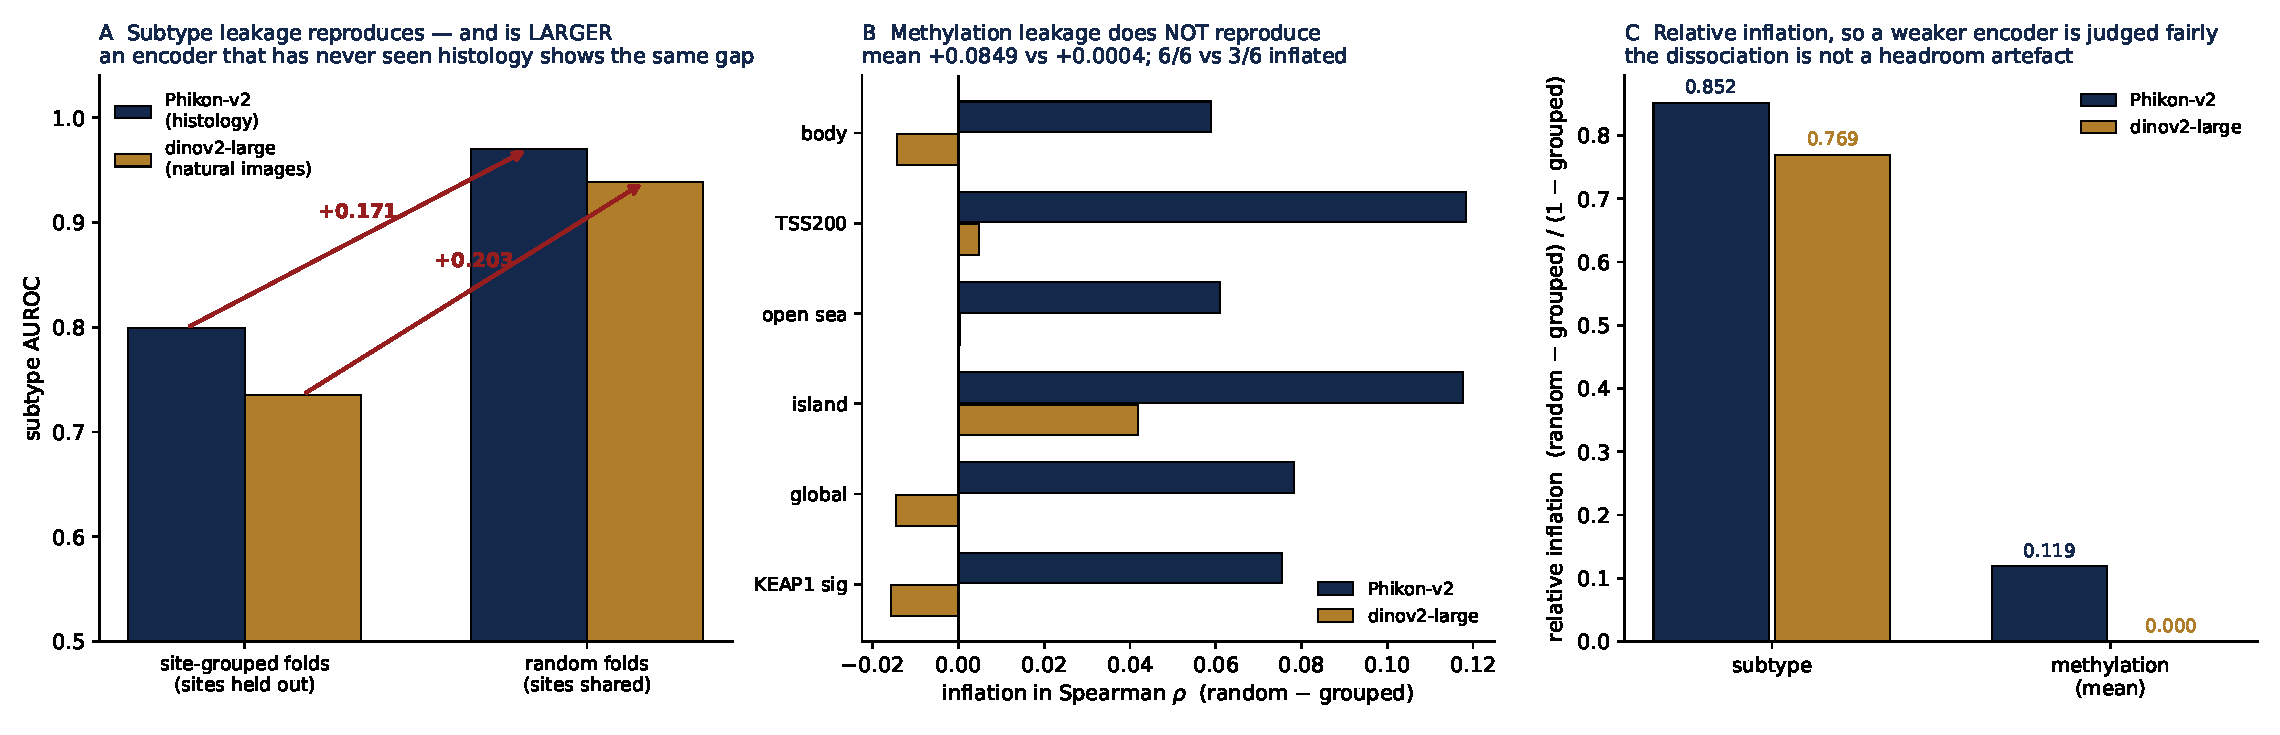
\includegraphics[width=\textwidth]{r18_panels.pdf}
\end{center}
\noindent{\small\color{qgrey}\textbf{A} Subtype, both fold regimes, both encoders.
\textbf{B} Per-target methylation inflation. \textbf{C} The dissociation on relative
inflation, so the weaker encoder is judged on fraction-of-headroom rather than raw gap.}

\section{Limitations}

\textbf{Two encoders is not a survey.} This distinguishes "a property of Phikon-v2" from "a
property of the archive". It does not establish how the signature behaves across the pathology
foundation-model field. UNI, H-optimus-0 and Virchow2 are gated behind licence acceptance that was
not ours to give.

\textbf{The contrast is corpus, and also patch size.} \texttt{facebook/dinov2-large} uses patch 14 against
Phikon-v2's 16, so at 224\,px it sees 256 tokens rather than 196. Architecture class, width, depth,
objective, readout and normalisation are matched; patch size is not, and it cannot be without
retraining one of them.

\textbf{Absolute performance is not the point and should not be quoted as a comparison of
encoders.} A natural-image model doing worse at lung subtype than a histology model is expected
and uninteresting. The claim concerns the \emph{gap} between fold regimes within each encoder.

\textbf{One cohort.} TCGA lung, the same 760 patients, the same 67 sites, the same slides.

\section*{Reproducing this report}

\texttt{evidence/m16\_encoder\_compare\_analysis.py} (the analysis),
\texttt{evidence/mil\_encoder\_compare.py} (the eight arms),
\texttt{evidence/encode\_dinov2.py} (the encoder, pinned revision),
\texttt{evidence/config.yaml} (pre-declared rules, SHA-256
\texttt{143b3b9d0a92fabb\ldots}),
\texttt{evidence/gates.json}, \texttt{evidence/results.json},
\texttt{evidence/arms/} (the eight raw arm JSONs).
This document: \texttt{python3 make\_report.py}.

\end{document}
